\subsection{Aprendizado profundo}

O aprendizado profundo é uma área do aprendizado de máquina caracterizada por utilizar dados brutos como entrada e descobrir as representações necessárias para permitir o mapeamento adequado e assim tornando as soluções mais simples \apud{marti2017aprendizado}{lecun2015deep}.

Segundo \citeonline{lecun2015deep}, o aprendizado profundo são métodos de representação de aprendizado com vários níveis, obtidos por meio da decomposição de módulos simples e lineares, que transformam a representação de um nível em uma representação mais alta e abstrata. Por exemplo a representação de uma imagem é transformada em informações que identificam objetos.

Dividindo um problema complexo em problemas menores torna os métodos especializados, viabilizando tarefas mais complexas, depois essas tarefas que foram dividias são recombinadas e é gerado uma solução do problema \cite{marti2017aprendizado}.

Utilizando o exemplo anterior, reconhecimento de imagem, cada um desses métodos especializados seria responsável por reconhecer uma parte da imagem, como bordas, objetos, tamanho, etc. E após a junção desses métodos é feito a predição da imagem \cite{marti2017aprendizado}.

A principal diferença entre uma rede neural convencional e uma rede neural profunda é a quantidade de camadas, uma rede neural profunda possui varias camadas de processamento \apud{marti2017aprendizado}{haykin1999neural}.

\begin{figure}[H]
	\centering
	\caption{Comparação de uma rede neural convencional com uma rede neural profunda.}
	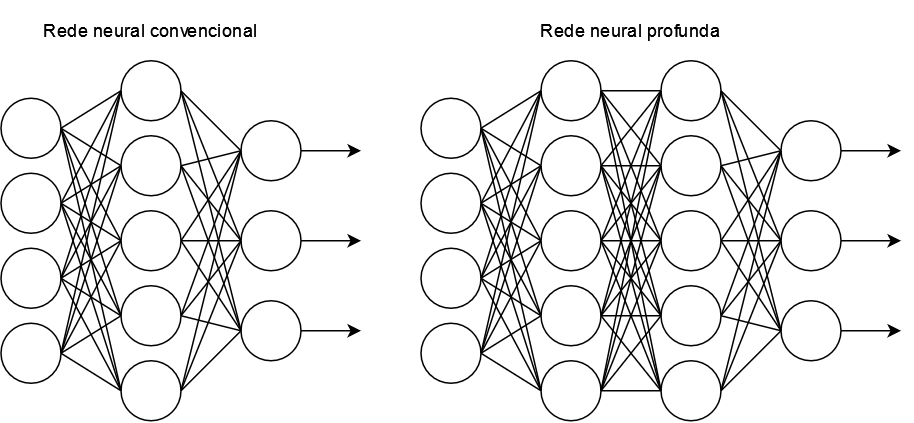
\includegraphics[width=0.8\textwidth]{figures/redes_neurais.png}
	\legend{Fonte: Criação propria}
	\label{fig:redes_neurais}
\end{figure}
